\flushleft \chapter{Zespołowe przedsięwzięcie}

\begin{itemize}
\item Zespołowe przedsięwzięcie inżynierskie oznaczać będzie projekt, działanie podjęte w realizacji postawionego celu, realizowane zespołowo.

\item Projekt jest odpowiedzią na problem/potrzebę, w określonej przestrzeni życia.
\end{itemize}

\section{Członkowie zespołu z określeniem funkcji}
\begin{description}
\item[1] Krzysztof Szabla - kierownik zespołu
\item[2] Mateusz Kempa - programista 
\item[3] Robert Dudzik - programista
\item[4] Adam Walczak - testujący
\end{description}

\section{Uzasadnienie potrzeby realizacji projektu}

Projekt obejmuje stworzenie aplikacji GPS na Androida, która poprowadzi członków spółki leśnej do oznaczonego drzewa, przeznaczonego do wycinki. Głownym problemem dla członków spółki leśnej jest kłopot ze znalezieniem trasy dojścia do danego drzewa, które wcześniej oznaczyli. Program ma powstać w celu uwydatnienia pracy spółki leśnej, członkowie będą wprowadzać punkty, czyli współrzędne oznaczonych drzew,  na podstawie których aplikacja będzie kierować ich w odpowiednie miejsce. Ich praca zostanie wykonana znacznie szybciej. Odpowiedzią na  rozwiązanie problemu będzie zespołowo zrealizowany projekt, którego wynikiem końcowym będą: program i sporządzona dokumentacja.

\section{Cele projektu} 

 Zespołowe Przedsięwzięcie Inżynierskie obejmuje stworzenie działającej aplikacji GPS na Androida, umożliwiającej poprawne i szybkie odnalezienie wyznaczonego celu. W tym przypadku celem jest określone drzewo, przeznaczone do wycinki, które należy oznaczyć odpowiednimi współrzędnymi, tak by członkowie spółki leśnej w łatwy sposób mogli je odnaleźć. Aplikacja ma wskazać trasę dojścia do oznaczonych wcześniej  obiektów..
 
 Główne cele:
 \begin{itemize} 
 \item zapoznanie się z zestawem Android SDK i odpowiednią literaturą przez programistów 
 \item wyszukanie podobnych do projektowanej aplikacji typu opensource i zapoznanie z nimi
 \item stworzenie działającej aplikacji i przetestowanie jej pod kątem zgodności z wytyczonymi zadaniami
 \item sporządzenie dokumentacji przez każdego członka zespołu na temat pracy jaką wykonał
 \end{itemize}

\section{Zakres projektu}
Zakres projektu obejmuje podzielenie obowiązków pomiędzy członków zespołu,  wyszukanie potrzebnych informacji i przygotowanie odpowiednich narzędzi. W celu rozpoczęcia pracy przy projekcie należy zapoznać się z literaturą i skorzystać z oprogramowania typu opensource w celu zapoznania się z kodem podobnych aplikacji. Do rozpoczęcia projektu potrzebne będą dwie rzeczy:Java Developer Kit, oraz zestaw Android SDK.  Android SDK zawiera kompilator programów na platformę Android, narzędzia do tworzenia i zarządzania wirtualnymi urządzeniami (na których możemy testować nasze programy), a także środowisko programistyczne Eclipse, JDK to  Java z narzędziami dla programistów (np. kompilator Javy).Zadaniem programistów jest napisanie programu, który zostanie przetestowany przez testera, by wyeliminować ewentualne błędy.
Projekt obejmuje także sporządzenie dokumentacji na temat wykonanej pracy.

\section{Grupy docelowe}

Głównymi odbiorcami i użytkownikami projektu są członkowie spółki leśnej, zajmujący się wycinką drzew.

\section{Struktura podziału prac (zadań) - WBS}

\begin{enumerate}
\item Wybór tematu projektu.
\item Wywiad ze zleceniodawcą i zebranie informacji na temat wymagań związanych z aplikacją.
\item Podzielenie zadań pomiędzy członków zespołu i zapoznanie z tematem.

- informacje o celu projektu

- informacje na temat działania programu

- informacje o wyniku, jaki ma być zwrócony przez program
\item Przygotowanie odpowiednich narzędzi i gromadzenie niezbędnych danych.

- przygotowanie środowiska Latex

- przygotowanie środowiska Android Studio
\item Napisanie programu.

-zaplanowanie interakcji pomiędzy poszczególnymi elementami aplikacji

-tworzenie algorytmów

-opis interfejsu

\item Testowanie programu i wprowadzanie ewentualnych zmian.
\end{enumerate}

\section{Diagram sieciowy}
Diagram sieciowy ukazuje zależności czasowe, węzły (aktywności), krawędzie (zależności czasowe).
\begin{figure}[H]
\centering
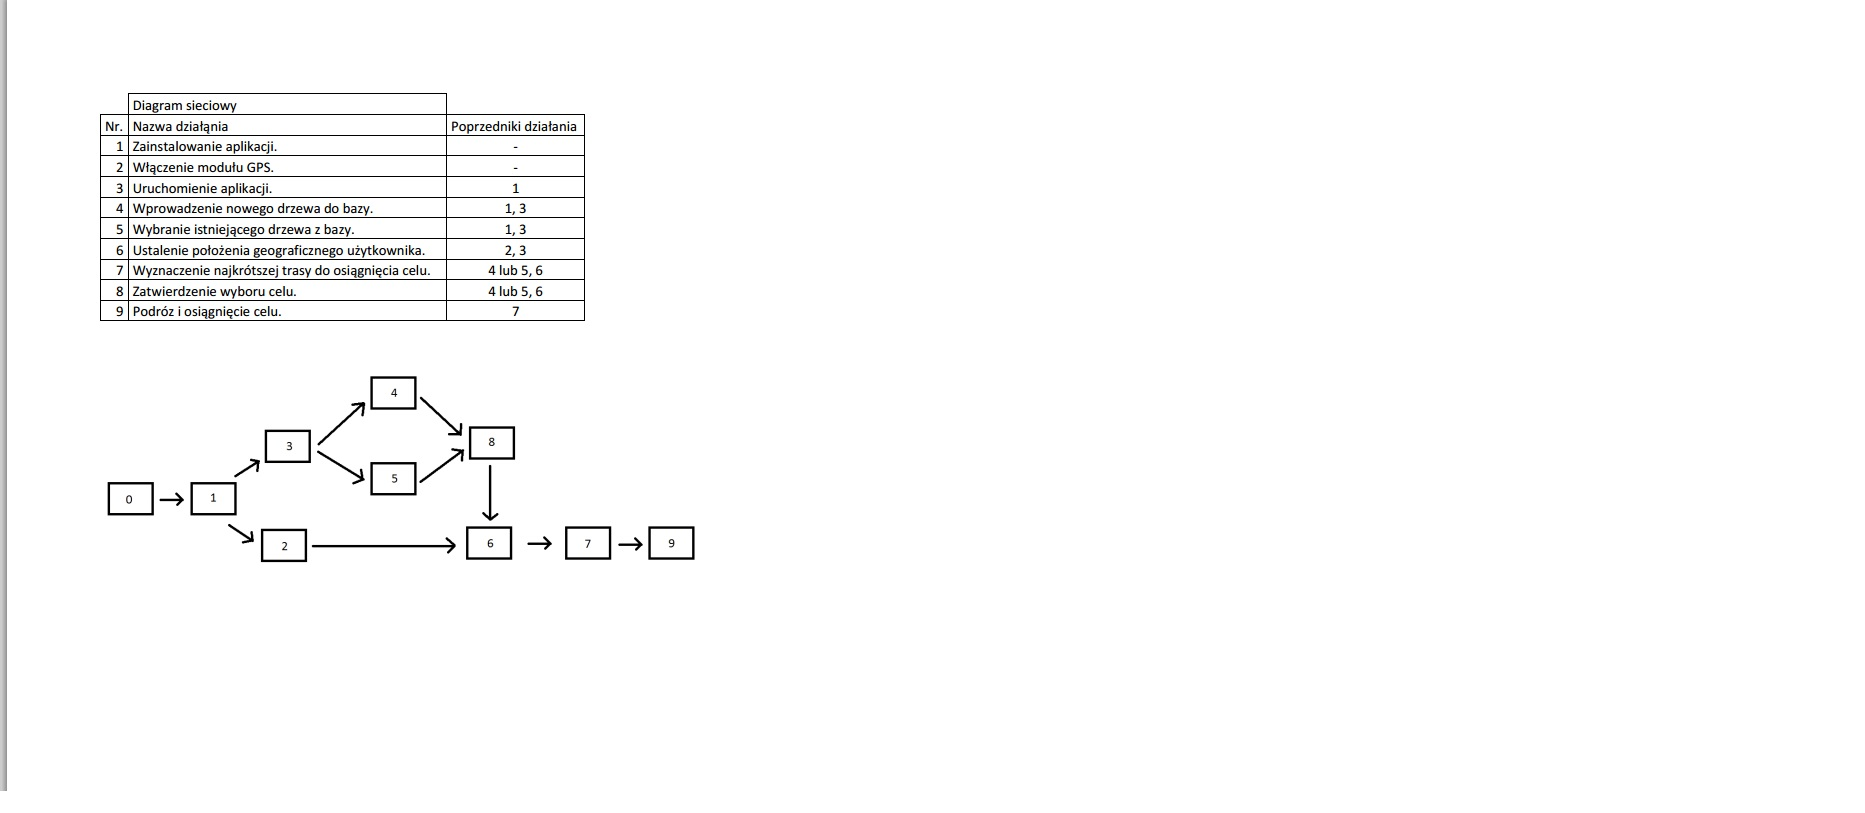
\includegraphics[scale=0.5]{czlonkowie/fig/diagram.jpg}
\end{figure}

\section{Harmonogram}
\begin{figure}[H]
\centering
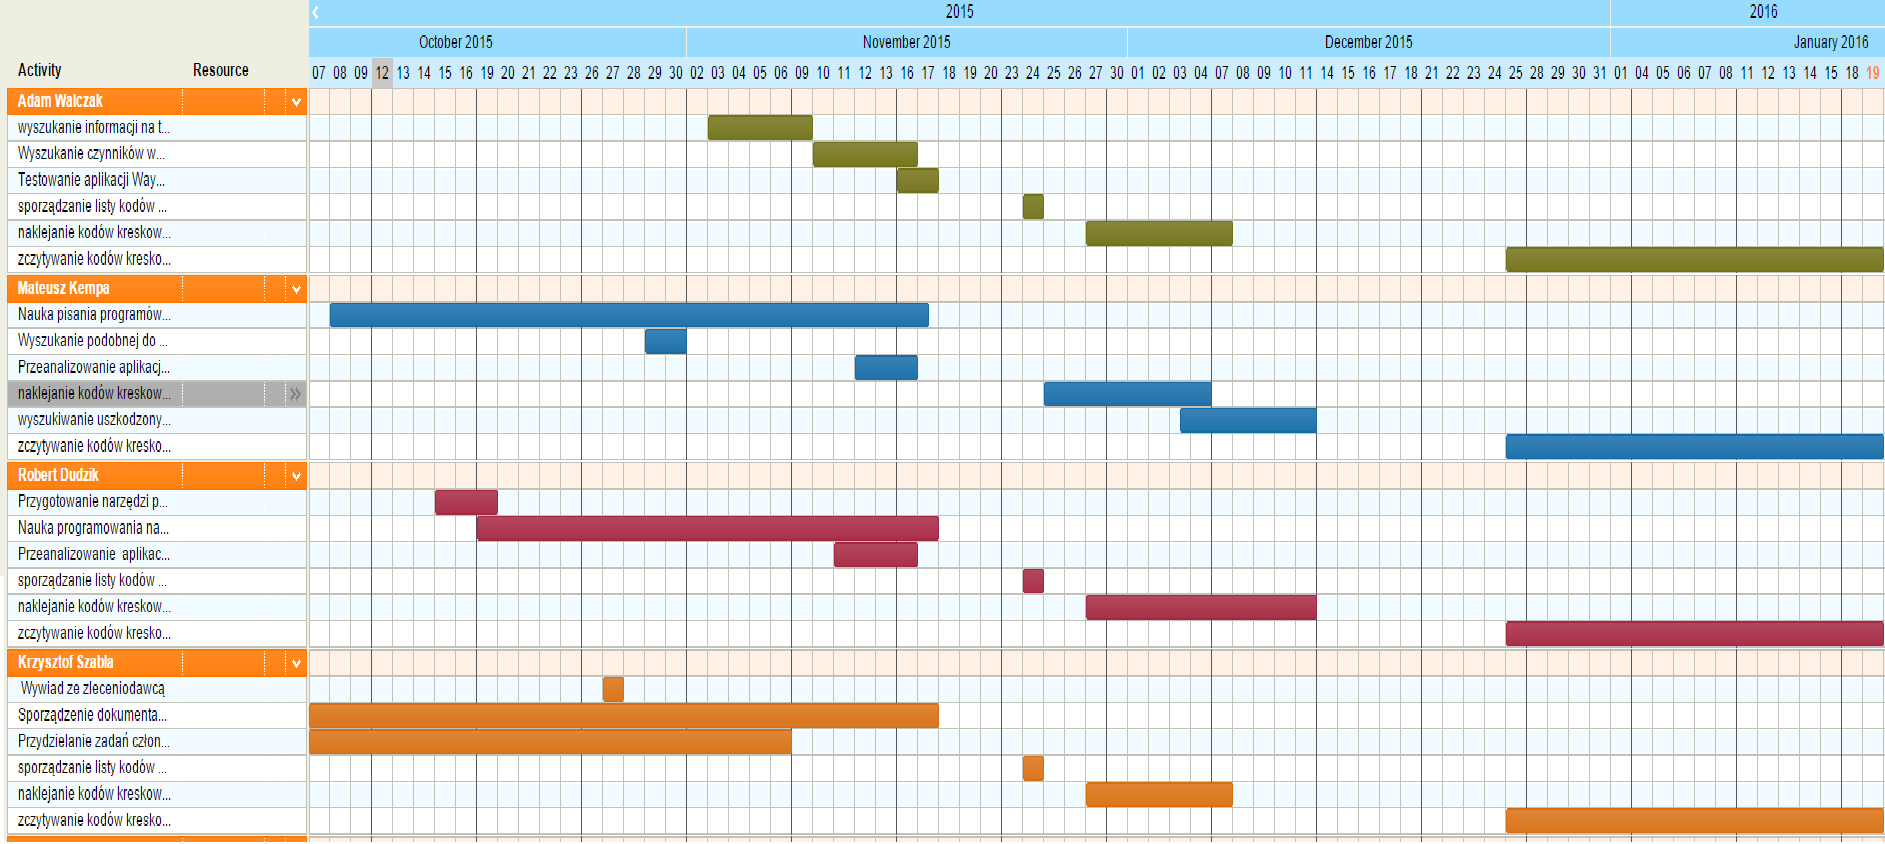
\includegraphics[scale=0.5219 , angle=90,]{czlonkowie/1/wykresGantta.png}

\end{figure}




\subsection{Harmonogram prac poszczególnych członków zespołu}

 Adam Walczak- tester. \newline
 
\textbf{GPS}
\begin{itemize}
\item Wyszukanie informacji na temat dokładności GPS-a.

\textbf{Data rozpoczęcia} 03.11.2015

\textbf{Data zakończenia} 10.11.2015
\item Wyszukanie czynników wpływających na wynik pomiaru GPS, wad i zalet GPS

\textbf{Data rozpoczęcia} 10.11.2015

\textbf{Data zakończenia} 16.11.2015
\item Testowanie aplikacji Waypoint w terenie.

\textbf{Data rozpoczęcia} 16.11.2015

\textbf{Data zakończenia} 17.11.2015
 \newline

\textbf{Biblioteka}
\item sporządzanie listy kodów kreskowych

\textbf{Data rozpoczęcia} 24.11.2015

\textbf{Data zakończenia} 24.11.2015

\item naklejanie kodów kreskowych na regałach  w czytelni

\textbf{Data rozpoczęcia} 27.11.2015

\textbf{Data zakończenia} 07.12.2015

\item zczytywanie kodów kreskowych książek w czytelni

\textbf{Data rozpoczęcia} 25.12.2015 

(w trakcie realizacji)

\end{itemize}

Mateusz Kempa- programista

\textbf{GPS}
\begin{itemize}
\item Nauka pisania programów na Androida


\textbf{Data rozpoczęcia} 08.10.2015

\textbf{Data zakończenia} 17.11.2015
\item  Wyszukanie podobnej do zadanej aplikacji, którą można wykorzystać przy projekcie.

\textbf{Data rozpoczęcia} 29.10.2015

\textbf{Data zakończenia} 31.10.2015

\item Przeanalizowanie aplikacji Waypoint i określenie w jakim stopniu będzie pomocna przy projekcie

\textbf{Data rozpoczęcia} 12.11.2015

\textbf{Data zakończenia} 16.11.2015

\item naklejanie kodów kreskowych na regałach  w czytelni

\textbf{Data rozpoczęcia} 28.11.2015

\textbf{Data zakończenia} 05.12.2015

\item wyszukiwanie uszkodzonych kodów kreskowych

\textbf{Data rozpoczęcia} 03.12.2015

\textbf{Data zakończenia} 12.12.2015

\item zczytywanie kodów kreskowych książek w czytelni

\textbf{Data rozpoczęcia} 25.12.2015 

(w trakcie realizacji)
 \end{itemize}
 
 
 Robert Dudzik- programista
 
 \textbf{GPS}
 
 \begin{itemize}
 \item Przygotowanie narzędzi programistycznych Android Studio
 
 \textbf{Data rozpoczęcia} 15.10.2015

\textbf{Data zakończenia} 19.10.2015

\item Nauka programowania na Androidzie na podstawie dostępnej literatury i stron internetowych

\textbf{Data rozpoczęcia} 19.10.2015

\textbf{Data zakończenia} 17.11.2015

\item Przeanalizowanie  aplikacji Waypoint i określenie w jakim stopniu będzie pomocna przy projekcie

\textbf{Data rozpoczęcia} 11.11.2015

\textbf{Data zakończenia} 16.11.2015


\textbf{Biblioteka}

\item sporządzanie listy kodów kreskowych

\textbf{Data rozpoczęcia} 24.11.2015

\textbf{Data zakończenia} 24.11.2015
\item naklejanie kodów kreskowych na regałach  w czytelni

\textbf{Data rozpoczęcia} 27.11.2015

\textbf{Data zakończenia} 11.12.2015

\item zczytywanie kodów kreskowych książek w czytelni

\textbf{Data rozpoczęcia} 25.12.2015

(w trakcie realizacji)
 \end{itemize}

Krzysztof Szabla- kierownik zespołu

\textbf{GPS}
\begin{itemize}

\item Wywiad ze zleceniodawcą

\textbf{Data rozpoczęcia} 27.10.2015

\textbf{Data zakończenia} 27.10.2015
\item Sporządzenie dokumentacji

\textbf{Data rozpoczęcia} 07.10.2015

\textbf{Data zakończenia} 17.11.2015

\item  Przydzielanie zadań członkom zespołu

\textbf{Data rozpoczęcia} 07.10.2015

\textbf{Data zakończenia} 06.11.2015

\textbf{Biblioteka}

\item sporządzanie listy kodów kreskowych

\textbf{Data rozpoczęcia} 24.11.2015

\textbf{Data zakończenia} 24.11.2015 



\item naklejanie kodów kreskowych na regałach  w czytelni

\textbf{Data rozpoczęcia} 28.11.2015

\textbf{Data zakończenia} 07.12.2015


\item zczytywanie kodów kreskowych książek w czytelni

\textbf{Data rozpoczęcia} 25.12.2015 

(w trakcie realizacji)


\end{itemize}

\section{Zmiana tematu}

Dnia 17 listopada nastąpiła zmiana tematu projektu. Przyczyną była duża trudność poprzedniego projektu i problemy programistyczne. Nowy temat to: ,,Nadanie cech lokalizacji książek,  znajdujących się w czytelni PWSZ w Nowym Sączu''. Dzięki jego realizacji, czytelnik po odnalezieniu książki w katalogu elektronicznym, będzie w stanie z dokładnością do półki, odnaleźć fizyczny egzemplarz książki. 

\section{Cele nowego projektu} 
~~~Zespołowe przedsięwzięcie inżynierskie obejmuje stworzenie systemu, który umożliwi czytelnikowi odnalezienie fizycznej lokalizacji książki wyszukanej w elektronicznym katalogu biblioteki PWSZ. 

~~~Na wstępie należy sprawdzić, jakimi czytnikami dysponuje czytelnia i wybrać kod kreskowy. W naszym projekcie używany będzie Code 39, ponieważ jest on obsługiwany przez czytniki znajdujące się w bibliotece oraz koduje znaki alfanumeryczne wraz ze znakami specjalnymi (takimi jak znak pauzy). Każdy kod będzie składał się z dwóch liczb całkowitych. Pierwsza to numer regału, a druga numer półki. Oddzielał je będzie znak '-'. Numeracja zaczyna się od '1-1' w górę, by w razie potrzeby można było rozbudować regał o kolejne półki. 

~~~Następnie trzeba będzie przygotować szablon kodów kreskowych, tak by były one odpowiedniej wielkości i jak najwięcej zmieściło się ich na jednej stronie. Na podstawie rozmiarów półek ustaliliśmy, że kody powinny mieć wysokość 13 mm, a margines z prawej strony wynosić 6 mm. Do utworzenia szablonu użyjemy programu Microsoft Excel oraz darmowej czcionki o nazwie "fre3of9x". 

~~~W dalszej kolejności zajmiemy się wydrukiem kodów. W tym celu użyjemy przygotowanego wcześniej szablonu, który będzie drukowany na specjalnym papierze samoprzylepnym w formacie A4. Dzięki temu w prosty sposób umieścimy kody na regałach. Po wydrukowaniu, kody zostaną pocięte przy pomocy biurowej gilotyny. 

\begin{figure}[H]
\begin{center}
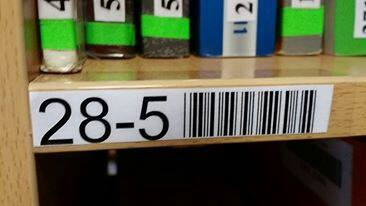
\includegraphics[scale=0.7]{czlonkowie/1/b2.jpg}
\caption{Przykładowy kod kreskowy}
\end{center}
\end{figure}
~~~Dalej konieczne będzie naklejenie kodów kreskowych. Umieszczać będziemy je z lewej strony półki, by później łatwo można było odczytać kody z poszczególnych książek. Każdy kod po przylepieniu musi zostać zabezpieczony przed fizycznym uszkodzeniem. Do tego wykorzystamy samoprzylepną folię ochronną, używaną w bibliotece do zabezpieczania książek lub dokumentów. Arkusz takiej folii zostanie podzielony na części o wymiarach 5x7 cm oraz 5x8.5 cm, w taki sposób aby przylepiona folia pokrywała w całości poprzednio naklejony kod. Niezwykle ważne będzie też sprawdzenie kodu już po jego zabezpieczeniu czy przypadkiem nie został on zamazany lub w jakikolwiek inny sposób uszkodzony. 

\begin{figure}[H]
\begin{center}
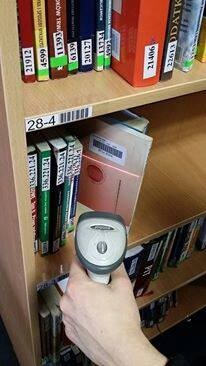
\includegraphics[scale=0.7]{czlonkowie/1/b1.jpg}
\caption{Zczytywanie kodów z książek}
\end{center}
\end{figure}

~~~Ostatnim celem naszego przedsięwzięcia jest odczytanie kodów kreskowych z książek w czytelni i przypisanie tych kodów do odpowiednich półek, w jak najbardziej efektywny sposób. Jest to jeden z najważniejszych etapów projektu. Do realizacji tego zadania posłuży nam czytnik Motorola LS2208 z interfejsem USB dostępny w bibliotece. Pozwala on odczytać kod i automatycznie zapisać go do pliku tekstowego. Kody kreskowe, które będziemy czytać znajdują się zwykle w lewym górnym rogu na tylnej stronie okładki książki. Kody te zostaną zapisane w formie listy, w notatniku. Jeśli którejś z książek nie będzie w danym momencie na półce, bo korzystali z niej czytelnicy, zostanie ona później uzupełniona przez pracowników biblioteki.
Należy tutaj sprecyzować znaczenie "najbardziej efektywnego sposobu". Nasza grupa ma za zadanie opracować system odczytu kodów, który pozwoli zrealizować ten cel w najkrótszym możliwym czasie, jednocześnie zachowując poprawność skanowanych kodów w pliku tekstowym. Opiszmy więc sposób zczytywania, który będzie sposobem optymalnym. Nasz zespół liczy czterech członków. Zakładając, że dysponujemy dwoma laptopami oraz skanerami podzielimy go na dwuosobowe podzespoły. W każdym podzespole jedna osoba zajmować się będzie zczytywaniem kodów, a druga kontrolą błędów w pliku tekstowym. Zczytywanie będzie się odbywać w następujący sposób. Najpierw pierwsza osoba skanowanć będzie kod półki, a później, od lewej strony wszystkie książki znajdujące się na poszczególnej półce. Przykładowy fragment pliku .txt będzie więc wyglądać tak: 
\begin{lstlisting}
88-1
88-2
0490000060045
0490000054227
0490000060046
0490000060036
0490000073645
0490000060047
0490000058234
0490000047888
0490000054041
88-3
0490000071851
0490000059162
\end{lstlisting}
Jak widzimy w pierwszym wierszu znajduje się kod półki '88-1'. Na tej półce nie znajdują się żadne książki, więc w kolejnym wierszu pojawia się kod następnej półki. Pod nim lista książek z owej półki. Dalej plik jest uzupełniany w podobny sposób. W tym samym czasie  druga osoba musi nieustannie monitorować zczytywane kody w pliku tekstowym, aby w razie nieudanego/niepoprawnego odczytu można było go powtórzyć. Druga podgrupa, wykorzystując identyczną metodę, zczytuje kody z innego regału. Warto w tym miejscu wspomnieć o pomiarach, które wykonaliśmy. Uśredniony czas zczytywania kodów z jednej półki wyniósł: 55.5 sekundy, natomiast jednego regału:5 minut 30 sekund.
Testowaliśmy również inny system skanowania, który w skrócie wyglądał tak: trzyosobowa grupa pracowała razem, pierwsza osoba zdejmowała i układała książki na półkach, druga zczytywała kody, a trzecia kontrolowała poprawność w pliku tekstowym. Średni czas skanowania półki dla tego sposobu to: 64.55 sekund, a regału: 6 minut 24 sekundy
Łatwo zauważyć, iż pierwszy system zczytywania jest lepszy od drugiego, bo:
\begin{itemize}
\item Jest on przeznaczony dla czteroosbowej grupy, tak więc wykorzystamy jej potencjał w pełni
\item Średni czas skanowania jest mniejszy - metoda jest szybsza
\item Dwie podgrupy pracują równolegle co znacznie skróci czas wykonywania zadania.
\end{itemize}
Jedyną zaletą drugiego systemu jest szybsze skanowanie książek na przepełnionych półkach, problematycznych w skanowaniu dla jednej osoby.

\section{Zakres nowego projektu}
Zakres nowego projektu obejmuje:

\begin{enumerate}
\item Wybór kodu kreskowego, który zostanie wykorzystany do identyfikacji regałów w czytelni. 
\item Przygotowanie szablonu kodów kreskowych w ustalonym standardzie, gotowego do druku.
\item Przylepienie kodów kreskowych na półki w czytelni PWSZ. 
\item Odczytanie kodów kreskowych wszystkich książek znajdującyh się w czytelni i przypisanie ich do odpowiednich półek (regałów).
 \end{enumerate}

\section{Grupy docelowe nowego projektu}

W nowym projekcie głównymi odbiorcami i użytkownikami są pracownicy  biblioteki oraz czytelnicy.

\section{Struktura podziału prac (zadań) - WBS dla nowego projektu}
\begin{enumerate}
\item Otrzymanie nowego tematu projektu.
\item Wywiad ze zleceniodawcą i zebranie informacji na temat wymagań związanych z projektem
\item Podzielenie zadań pomiędzy członków zespołu i zapoznanie z tematem.
\item Przygotowanie listy kodów kreskowych oraz numeracji poszczególnych półek i regałów
\item Naklejanie kodów kreskowych na regały w czytelni i zabezpieczanie ich za pomocą folii ochronnej
\item Odczytywanie kodów kreskowych książek i przypisywanie ich do odpowiedniej półki
\end{enumerate}

\section{Dokumentacja}
Przygotowanie środowiska do równoległego opracowania dokumentacji projektu i realizacji przydzielonych zadań poszczególnym członkom zespołu projektowego.

\subsection[Edycja plików dokumentacyjnych]{Edycja plików dokumentacyjnych - każdy członek zespoły niezależnie}
Każdy z członków zespołu edytuje swój plik \LaTeX{} (czlonkowie/nrCzlonka/main.tex) i~umieszcza w nim całość analiz i wyników, które pozwoliły mu zrealizować przydzielone zadanie. Wszystkie pliki graficzne, każdy niezależnie umieszcza w swoim katalogu (czlonkowie/nrCzlonka).

Pierwszą linia w pliku (czlonkowie/nrCzlonka/main.tex), zawiera imię i nazwisko opracowującego członka zespołu:
\begin{lstlisting}
\osoba{Robert Dudzik}
\end{lstlisting}

Każde działanie/zadanie należy DOKŁADNIE opisać podając w poleceniu \s!\zadanieprojektowe! cztery obowiązkowe dane:
\begin{itemize}
\item Rodzaj zadania [Przygotowanie przestrzeni do zespołowej pracy]
\item Data rozpoczęcia [2015-10-06]
\item Data zakończenia [2014-11-02]
\item Aktualny status [zaplanowane do realizacji]
\item dokładny opis realizowanego zadania [powinien zawierać opis, rysunki, tabele, kody napisanych programów]
\end{itemize}

Poniżej znajduje się przykładowy listing dla skróconych dwóch zadań:
\begin{lstlisting}
\zadanieprojektowe{Przygotowanie dokumentacji}{2014-11-01}{2014-11-02}{w trakcie do realizacji}

Poniżej opisujemy całe zadanie zgodnie z konwencją poznaną na NI.
Poniżej opisujemy całe zadanie zgodnie z konwencją poznaną na NI.

Poniżej opisujemy całe zadanie zgodnie z konwencją poznaną na NI. 

%następne zadanie
\zadanieprojektowe{Przygotowanie dokumentacji}{2014-11-03}{2014-11-03}{zakończone}
\begin{figure}[H]
\includegraphics[width=\textwidth]{czlonkowie/1/studzienkizDziura.jpg}
\end{figure}
\end{lstlisting}


\subsubsection{Obsługa SVN}
Umieszczanie w repozytorium plików lub katalogów dotychczas nie podlegający zarządzaniu wersjami.

Użycie: import [ŚCIEŻKA] URL

Rekurencyjnie kopiuje ŚCIEŻKA do URL. Jeśli ŚCIEŻKA nie jest podana, domyślną wartością jest '.'. W repozytorium są w razie potrzeby tworzone brakujące katalogi nadrzędne. Jeśli argument ŚCIEŻKA jest katalogiem, to zawartość katalogu jest dodawana bezpośrednio za URL-em.

Przydatne parametry:

-m ARG  -  użyj podanego tekstu jako opisu zmian

--username ARG  : użyj ARG jako nazwy użytkownika

--password ARG  : użyj ARG jako hasła

Tworzenie kopii roboczej projektu

Użycie: checkout URL[@WERSJA]... [ŚCIEŻKA]

Pobiera dane z URL i umieszcza je w ŚCIEŻKA.

Dodawanie i aktualizacja plików/katalogów

Użycie: commit [ŚCIEŻKA...]

Zatwierdza zmiany dokonane na kopii roboczej zapisując je w repozytorium. ŚCIEŻKA wskazuje pliki/katalogi z kopii roboczej, które mają być uaktualnione w repozytorium.

Aktualizacja kopi roboczej projektu

Użycie: update [ŚCIEŻKA...]

Aktualizuje kopię roboczą nanosząc zmiany obecne w repozytorium.  Jeśli nie podano wersji, nanoszone są najnowsze zmiany z  repozytorium (wersja HEAD).

\subsection{Github}
\subsubsection{Połączenie z siecią}
Github nie wymaga podłączenia do sieci. Można mieć repozytorium lokalne i w nim \verb|commitować| swoje zmiany. Ale jeśli chce się żeby ktoś inny z nich skorzystał, to i tak trzeba zrobić \verb|pusha|. Lokalne commity pozwalają nam cofnąć się do poprzednich wersji, a \verb|push| używamy na mając skończony fragment kodu. 

\subsubsection{Tworzenie nowego repozytorium}
Korzystając z GitHuba możesz z jego poziomu stworzyć nowe repozytorium i sklonować lokalnie na dysku przez polecenie \texttt{git clone https://github.com/<twój-login>/ test.git} (możesz na końcu dodać parametr wskazujący katalog, do którego zostanie sklonowany projekt, czyli \texttt{git clone <adres-repo> katalog}). Teraz możesz pracować na plikach i synchronizować swoją wersję z wersją zdalną.
Alternatywnie możesz zacząć pracować lokalnie (uruchomienie w katalogu projektu polecenia \verb|git init|). Będziesz mógł korzystać lokalnie z wersjonowania plików. Aby zsynchronizować projekt do zdalnego repozytorium, musisz założyć puste repozytorium (np. we wspomnianym GitHubie), a następnie lokalnie uruchomić polecenie git remote add test \texttt{https://github.com/<twój-login>/test.git}, a następnie zsynchronizować lokalny projekt do zdalnego repozytorium przez git \texttt{push origin master}.

\subsubsection{Dodawanie, usuwanie i modyfikacja plików}
Aby dodać plik, musisz go oczywiście stworzyć. Dodawanie istniejącego pliku do repozytorium wykonuje się poleceniem \verb|git add <plik>|. Aby usunąć plik istniejący w repozytorium, należy użyć polecenia \verb|git rm <plik>|. Po zmodyfikowaniu pliku nie musisz wykonywać żadnych poleceń, przy \verb|commicie| wystarczy parametr aby pliki zmodyfikowane, dodane i usunięte automatycznie znalazły się w commicie.
Aby zobaczyć jakie dodane, usunięte i zmodyfikowane pliki oczekują na zatwierdzenie (\verb|commit|), oraz zobaczyć jakie pliki nie zostały dodane do repozytorium lokalnie, użyj polecenia \verb|git status|, lub \verb|git status -s|. To drugie wyświetla status w wersji short, czyli znacznie skróconej.
Jeśli chcesz sprawdzić, jakie zmiany zostały wykonane na plikach które chcesz zatwierdzać, użyj polecenia \verb|git diff| (jeśli chcesz zobaczyć zmiany we wszystkich plikach), lub \verb|git diff <plik>| (zmiany w jednym wybranym pliku).

\subsubsection{Zatwierdzanie zmian}
Aby po zmianach w plikach zrobić nową kopię, należy użyć polecenia \verb|git commit -a|. Parametr -a powoduje, że pliki zmodyfikowane, dodane (przez \verb|git add|) i usunięte (przez \verb|git rm|) będą automatycznie uwzględnione w tej rewizji. W otwartym edytorze należy wpisać komentarz zmian, które zostały wykonane w stosunku do poprzedniej rewizji (poprzedniego wykonania \verb|commita|).

\subsubsection{Synchronizacja z repozytorium zdalnym}
Aby dokonane wcześniej zmiany które zostały „zacommitowane” trafiły do zdalnego repozytorium, należy je tam wysłać przy pomocy polecenia \verb|git push|. Jeśli chcesz wcześniej sprawdzić, jakie zmiany zostaną wysłane, możesz użyć polecenia \texttt{git diff master origin/master}.
Oczywiście może się zdarzyć, że ktoś inny wysłał do zdalnego repozytorium swoje zmiany. Aby być na bieżąco z projektem, warto w miarę często aktualizować projekt danymi ze zdalnego repozytorium poleceniem \verb|git pull|.

\subsubsection{Konflikty przy pull i merge}
Oczywiście może się zdarzyć, że przy wykonaniu pull otrzymasz komunikat \texttt{Automatic merge failed; fix conflicts and then commit the result}. Oznacza to, że Twoje zmiany powodują konflikt z tymi, które wykonał ktoś inny. Musisz wtedy otworzyć dany plik, wykonać ręcznie modyfikacje, a następnie wykonać \verb|git add <plik>| i najlepiej od razu \verb|git commit|.
Jeśli przed wykonaniem\verb|merge| wiesz jakie będą konflikty, możesz podać parametr powodujący, że konflikty będą rozwiązywane przyjmując wersję którą masz lokalnie (\texttt{git merge -s ours origin/master}) lub przyjmując wersję ściągniętą ze zdalnego repozytorium (\texttt{git merge -s theirs origin/master}).